% !TeX spellcheck = en_US
\section{What would happen in Spain if, after 20 years of the vaccination, the effect of the vaccine disappear completely?}
In this section, we are going to simulate what would happen if the vaccine is protecting completely the vaccinated woman during $20$ years and suddenly, in the month after these $20$ year, she losses completely the protection and she becomes vulnerable to the HPV LR 6/11 and oncogenic HPV. In Figure \ref{fig:perdida_proteccion} we can see the evolution of the protection simulated for every vaccinated woman.

\begin{figure}[h!]
	\centering
	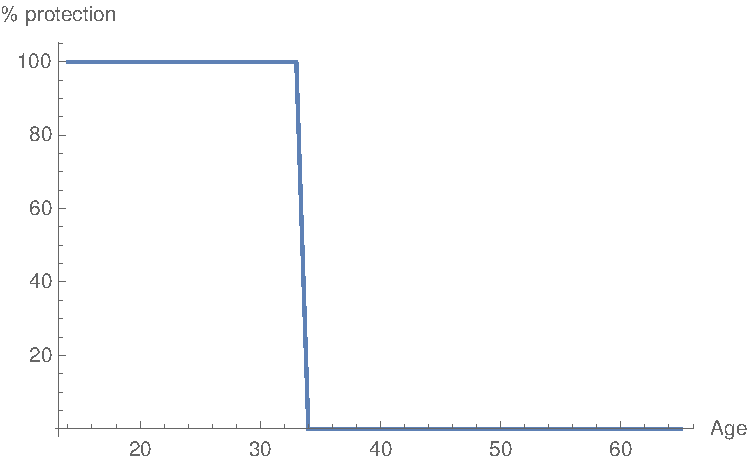
\includegraphics[width=0.5\linewidth]{IMGs/6.-Caida_brusca/grafica_perdida_proteccion.pdf}
	\caption{Evolution of the vaccine protection for every vaccinated woman. After vaccination until $20$ years, the vaccine protects completely ($100\%$) but the month after, the protection drops to $0\%$, the vaccine does not protect anymore.}
	\label{fig:perdida_proteccion}
\end{figure}

In Figure \ref{fig:dropLRESP}, we can see a comparative of the decline of HPV LR 6/11 between the scenario where the effect of the vaccine is permanent, shown in Sections \ref{sec:verr_spain} and \ref{sec:onco_spain}, and the scenario where the effect of the vaccine disappear completely after $20$ years. In the graphs for women and men we can see how this latter case stabilizes in levels of decline around $20\%$ lower, in average, than the case where the effect of the vaccine is permanent. However, a significant fraction of the population remains protected despite the loss of the protection. 

In regard to MSM, we can see that the lost of the vaccine protection does not affect the decline. This is a fact that also supports the statement that there is not herd immunity for MSM, even if the properties of the vaccine change, because the MSM decline does not change.

\begin{figure}[!]
	\centering
	\begin{tabular}{cc}
		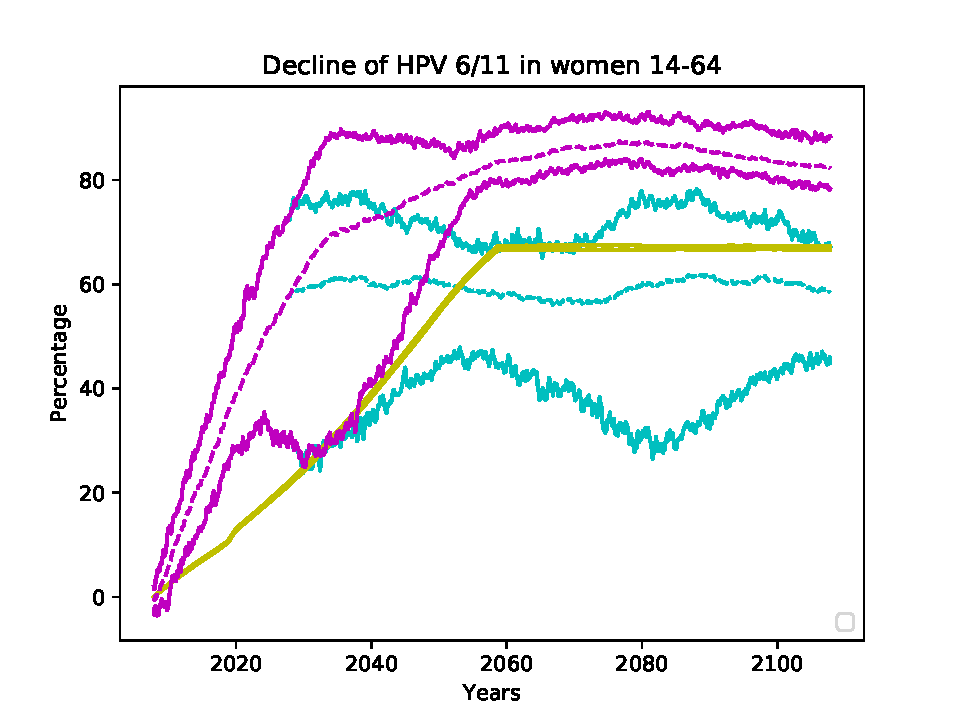
\includegraphics[width=0.5\linewidth]{IMGs/6.-Caida_brusca/verr_muj.pdf}	& 
		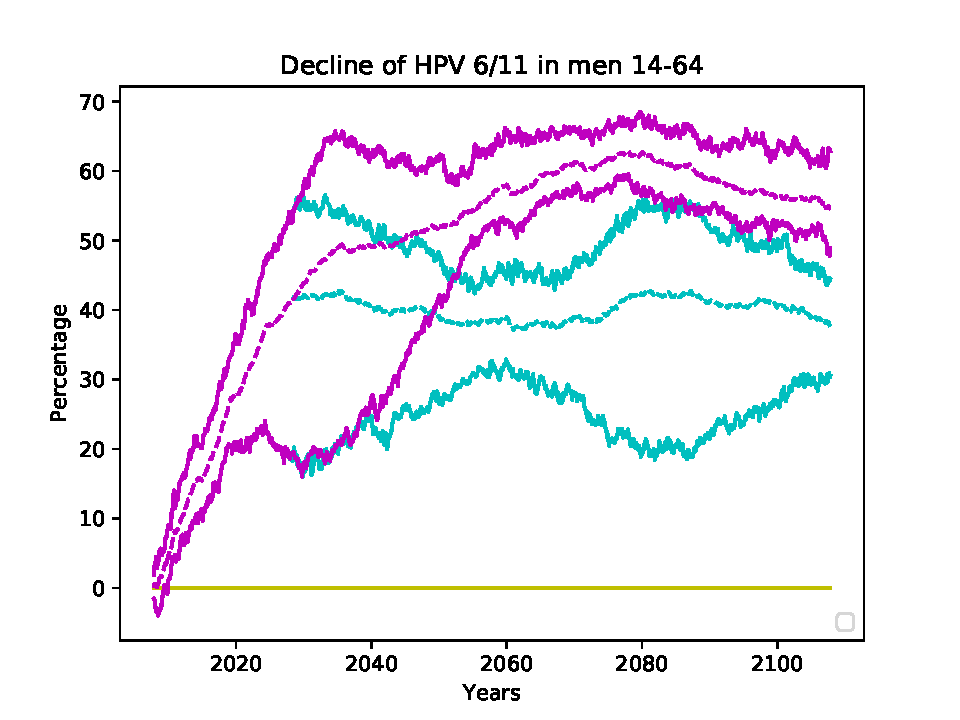
\includegraphics[width=0.5\linewidth]{IMGs/6.-Caida_brusca/verr_hom.pdf}  \\ 
		(a)	& (b) \\ 
		\multicolumn{2}{c}{ 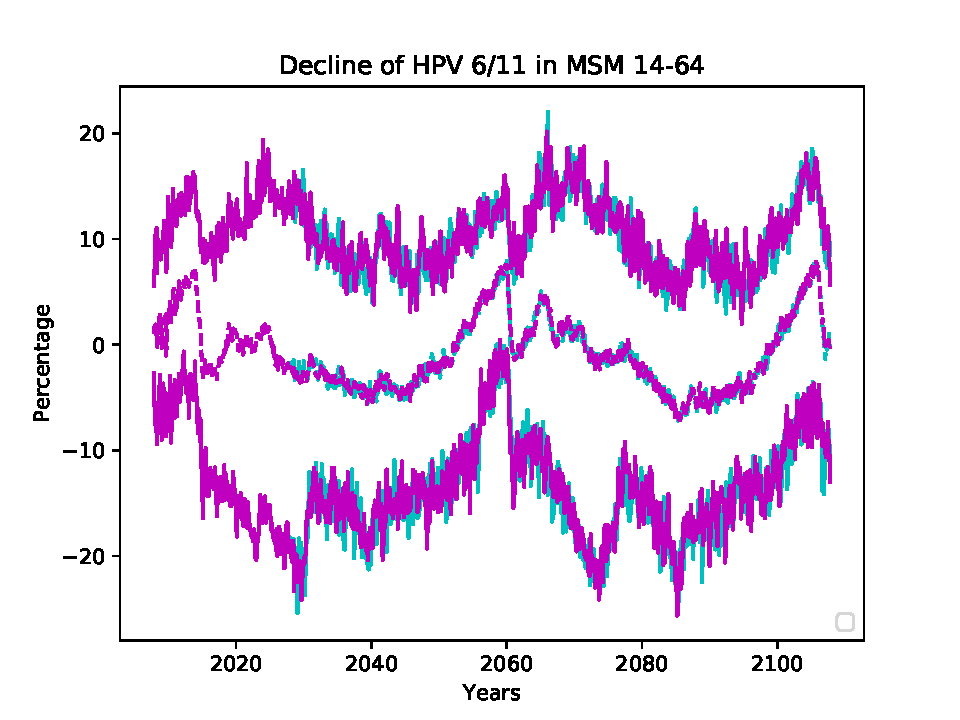
\includegraphics[width=0.5\linewidth]{IMGs/6.-Caida_brusca/verr_MSM.pdf} } \\ 
		\multicolumn{2}{c}{(c)} \\ 
	\end{tabular} 
	\caption{Comparative of the decline of HPV LR 6/11 in 14-64 years old women (a), men (b) and MSM (c) over the time, between the scenario where the effect of the vaccine is permanent (magenta lines, representing  the mean and the $95\%$ confidence interval) and the scenario where the effect of the vaccine disappear completely after $20$ years (cyan lines, representing  the mean and the $95\%$ confidence interval). As we can see, for women and men, the latter stabilizes in levels of decline about $20\%$ less, in average, than the case where the vaccine protects permanently. For MSM there are not changes between both scenarios.}
	\label{fig:dropLRESP}
\end{figure}

Now, in Figure \ref{fig:dropHRESP}, we can see an analogous comparative for the decline of oncogenic HPV between the mentioned scenarios: permanent protection and the drop of the protection after $20$ years. The graphs are very similar to the ones in Figure \ref{fig:dropLRESP} with the only change that the difference between the levels of decline are higher. The results for MSM are almost identical, what supports that there is not herd immunity effect on them.

\begin{figure}[!]
	\centering
	\begin{tabular}{cc}
		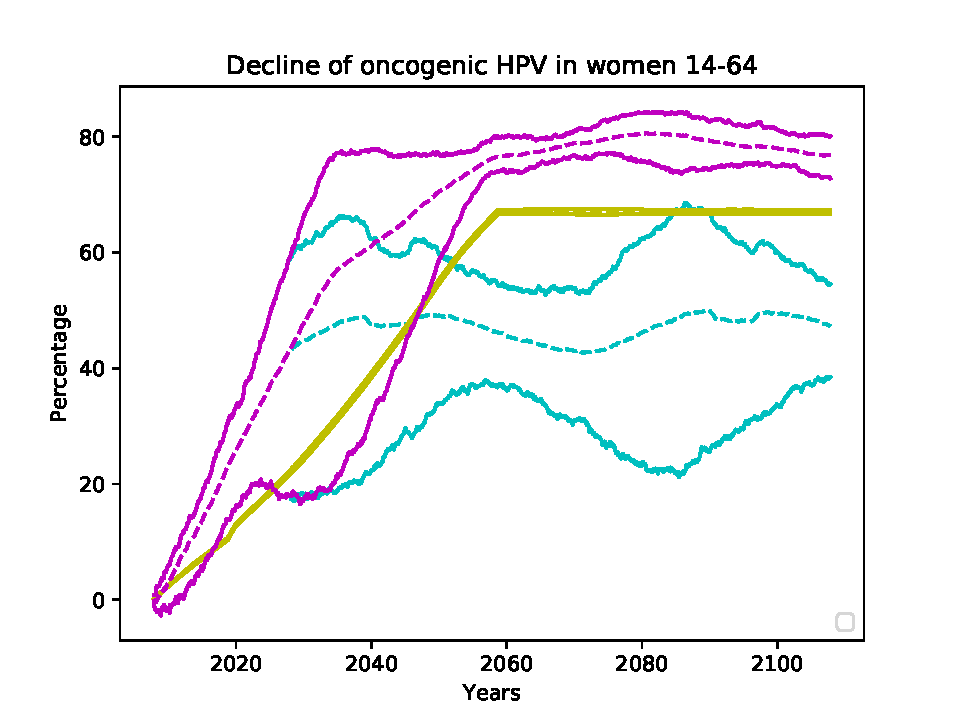
\includegraphics[width=0.5\linewidth]{IMGs/6.-Caida_brusca/onco_muj.pdf}	& 
		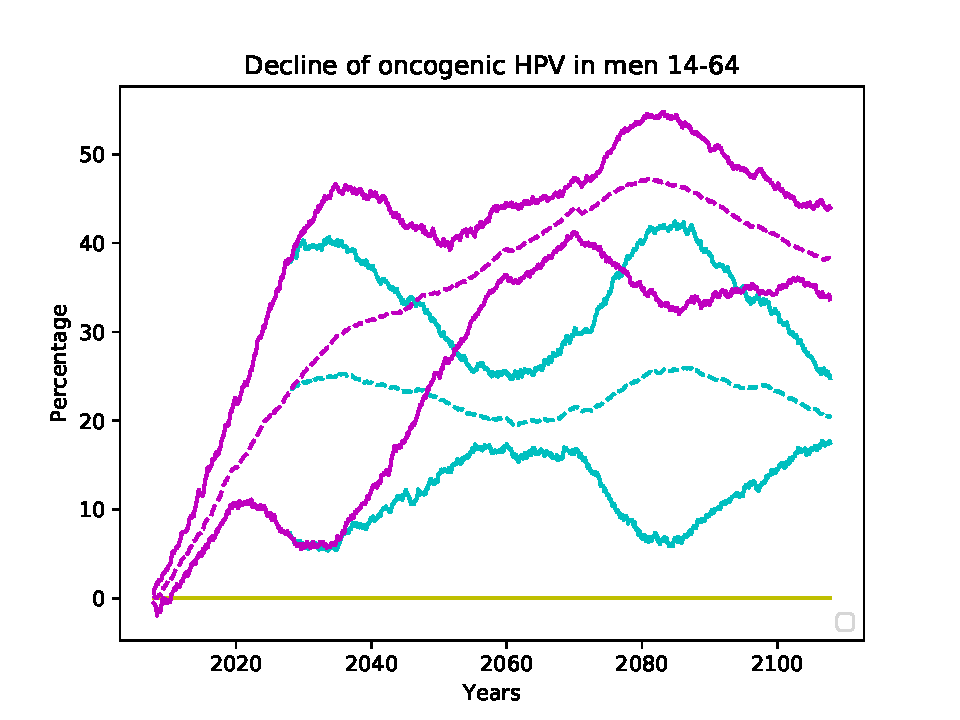
\includegraphics[width=0.5\linewidth]{IMGs/6.-Caida_brusca/onco_hom.pdf}  \\ 
		(a)	& (b) \\ 
		\multicolumn{2}{c}{ 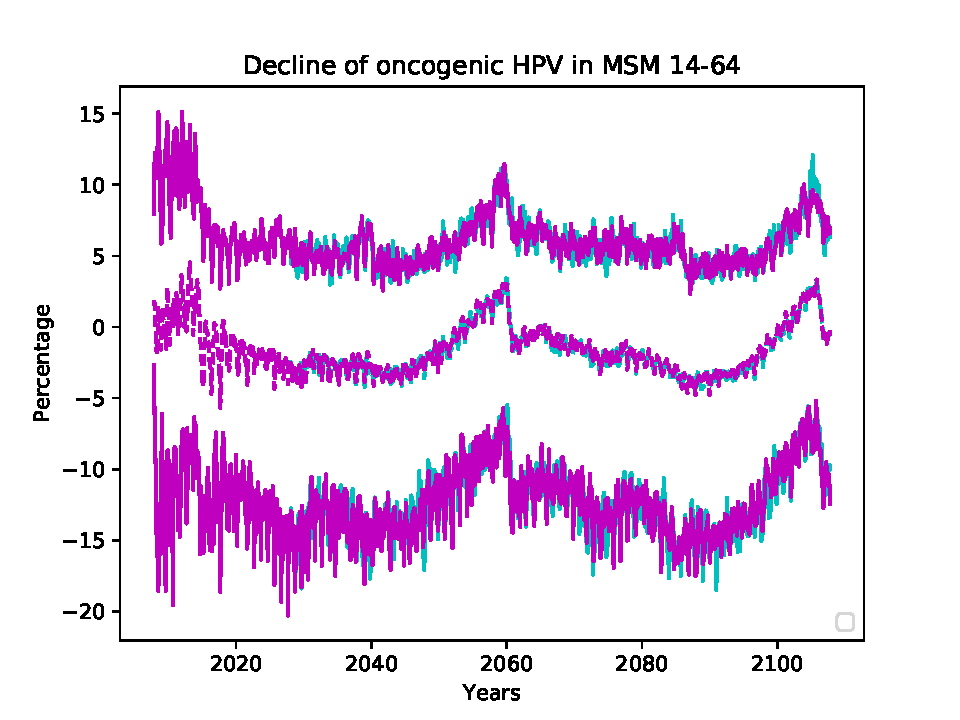
\includegraphics[width=0.6\linewidth]{IMGs/6.-Caida_brusca/onco_MSM.pdf} } \\ 
		\multicolumn{2}{c}{(c)} \\ 
	\end{tabular} 
	\caption{Comparative of the decline of oncogenic HPV infections in 14-64 years old women (a), men (b) and MSM (c) over the time, between the scenario where the effect of the vaccine is permanent (magenta lines, representing  the mean and the $95\%$ confidence interval) and the scenario where the effect of the vaccine disappear completely after $20$ years (cyan lines, representing  the mean and the $95\%$ confidence interval). The graphs are very similar to the ones in Figure \ref{fig:dropLRESP} with the only change that the difference between the levels of decline are higher. For MSM there are not changes between both scenarios.}
	\label{fig:dropHRESP}
\end{figure}

Now, we are going to perform a sensitivity analysis, consisting of the comparison between the decline of HPV infection if there is a drop in the vaccine protection after 20 years and after 30 years. This comparison will be done only for men and women, because there are not differences in MSM due to the lack of herd immunity effect. The results can be seen in Figure \ref{fig:compara_caida}.

\begin{figure}[!]
	\centering
	\begin{tabular}{cc}
		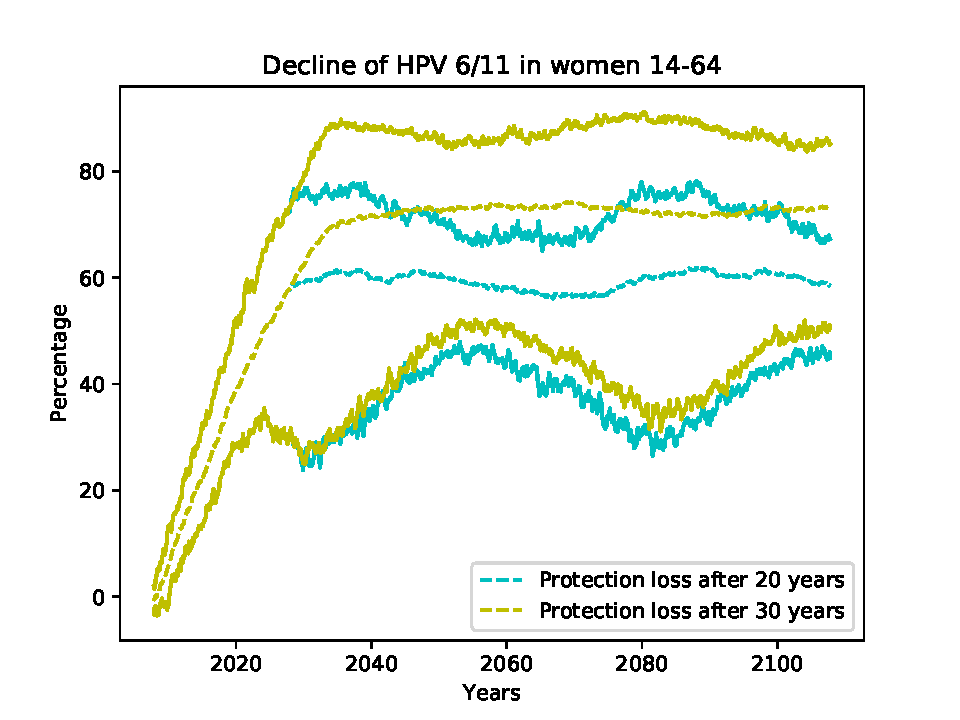
\includegraphics[width=0.5\linewidth]{IMGs/7.-Compara_caida/verr_muj.pdf}	& 
		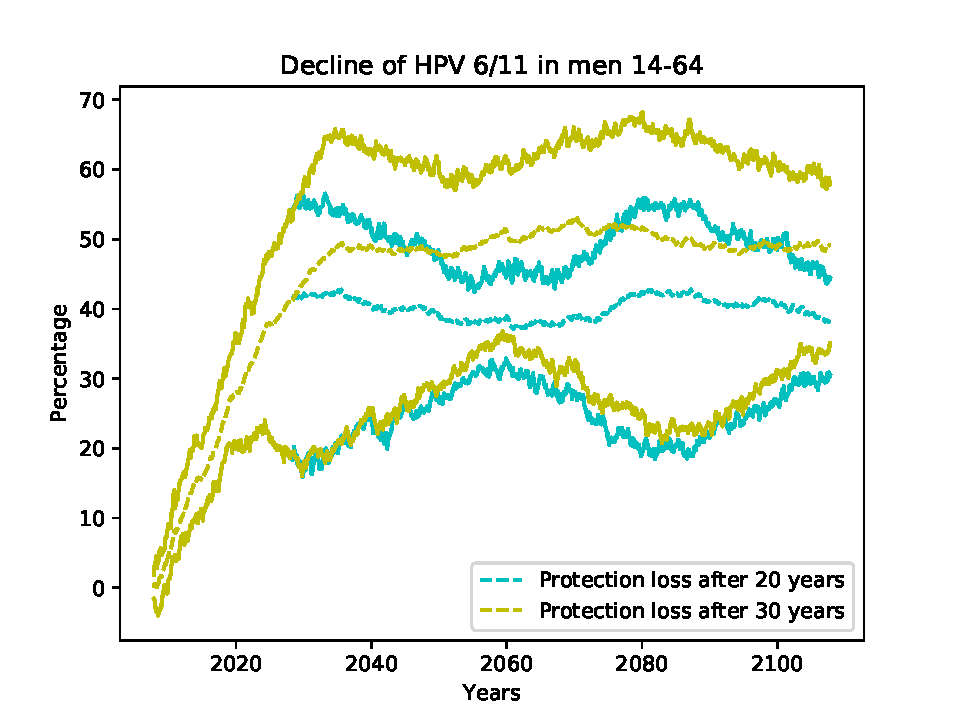
\includegraphics[width=0.5\linewidth]{IMGs/7.-Compara_caida/verr_hom.pdf}  \\ 
		(a)	& (b) \\ 
		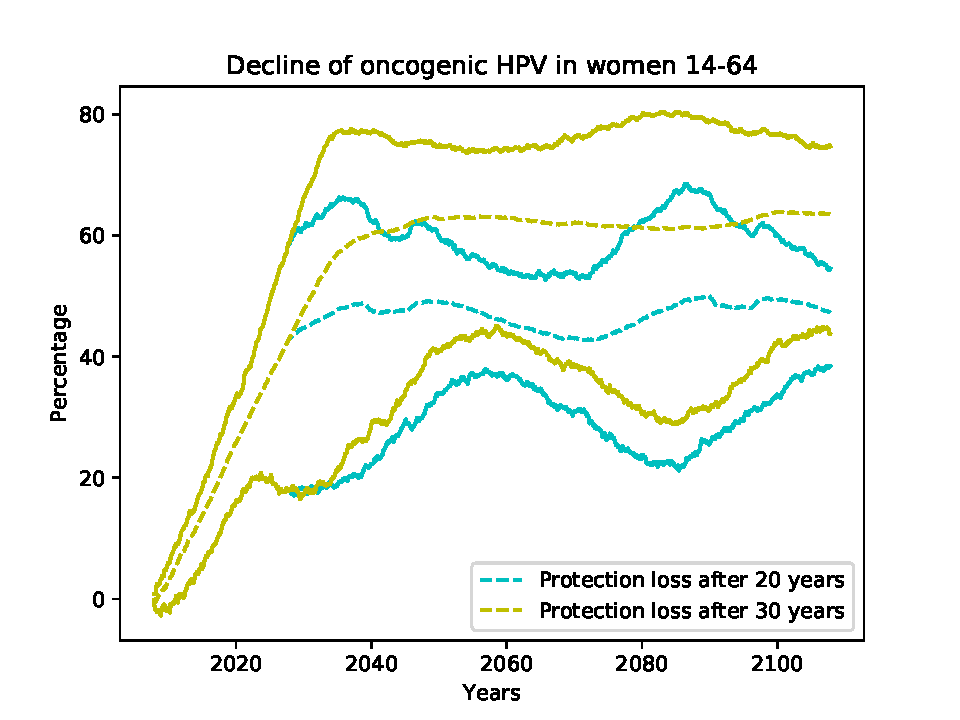
\includegraphics[width=0.5\linewidth]{IMGs/7.-Compara_caida/onco_muj.pdf}	& 
		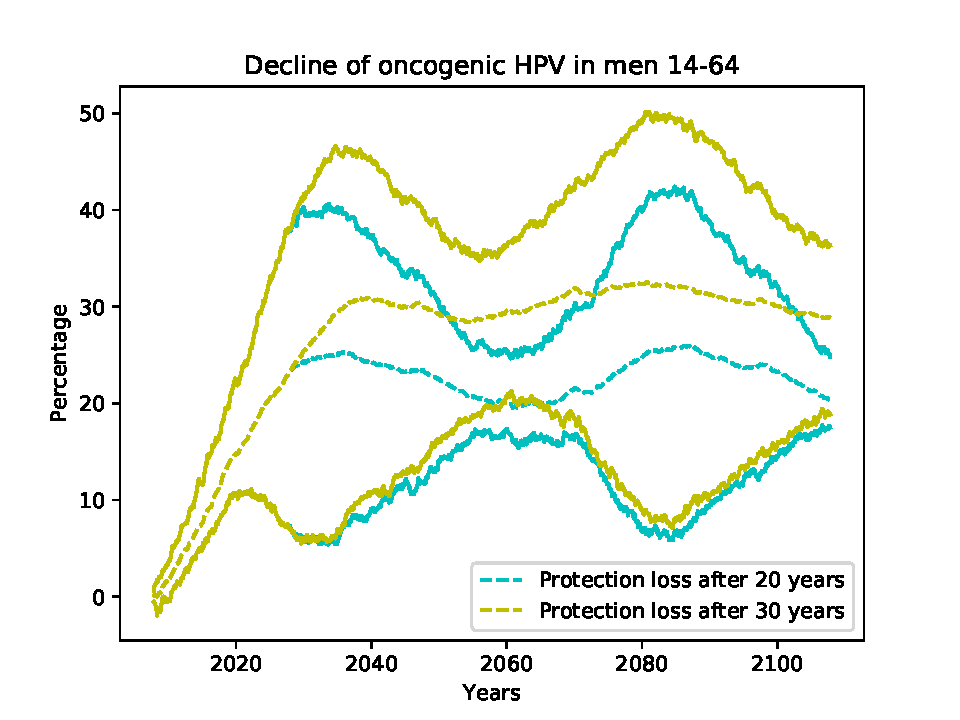
\includegraphics[width=0.5\linewidth]{IMGs/7.-Compara_caida/onco_hom.pdf}  \\ 
		(c)	& (d) \\ 
	\end{tabular} 
	\caption{Comparative of the decline of HPV 6/11 infections in 14-64 years old women (a) and men (b) over the time, between the scenario where the drop of the vaccine protection occurs after 20 years of vaccination (cyan lines) and after 30 years (yellow lines). The same for figures (c) and (d) with HPV oncogenic infection. The difference of 10 years in the drop results in around $10\%$ of difference in the decline.}
	\label{fig:compara_caida}
\end{figure}

Figure \ref{fig:compara_caida} leads us to conclude that the longer is the vaccine protection the lower will be the drop in the decline. 

To finish the present section, we are going to show Figure \ref{fig:proteccion} where we can see the percentage of women protected by the vaccine if the protection is permanent and if there is a loss of protection after 20 and 30 years.

\begin{figure}[!]
	\centering
	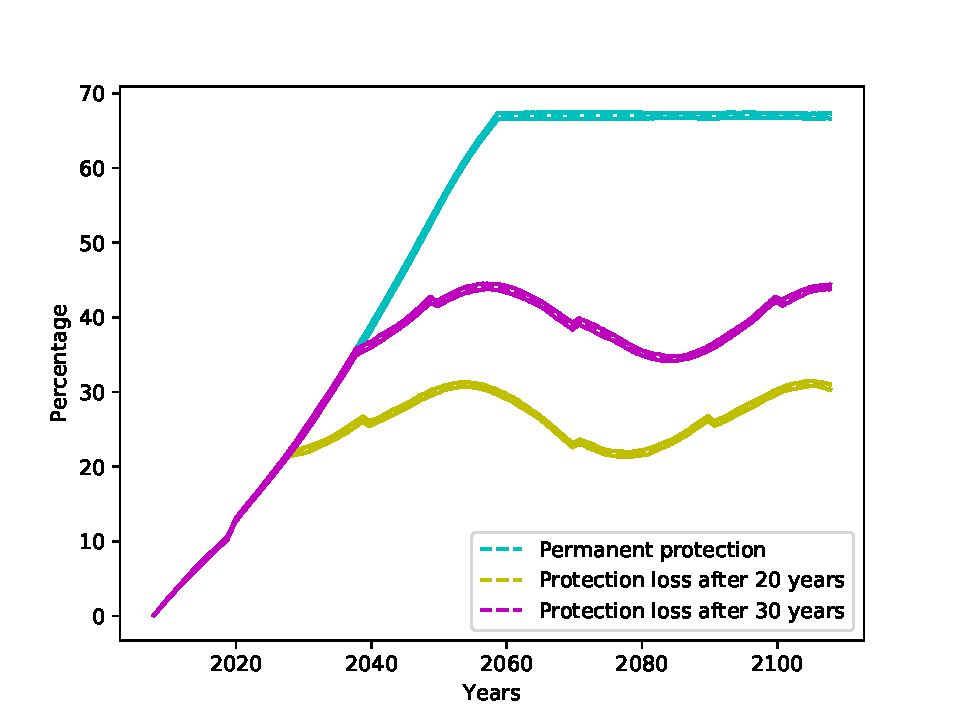
\includegraphics[width=0.5\linewidth]{IMGs/7.-Compara_caida/proteccion_muj.pdf}	
	\caption{Percentage of women protected by the vaccine in three scenarios: permanent protection (cyan line), total loss of protection after 30 years (magenta line) and total loss of protection after 20 years (yellow line).}
	\label{fig:proteccion}
\end{figure}

